\section{Results}

This chapter will present the transformed data we gathered while also showing visualization of said data. These visualizations conclude Tables and Figures.

\subsection{Architectural Comparison}

There is in every generation change also a change in the architectural structure of a RAM module and the chips. This way, generational changes can be possible. The most important architectural differences of DDR4 and DDR5 can be found in Table 1.

\begin{table}[H]
    \centering
    \begin{tabular}{|m{5cm}|P{3cm}|P{3cm}|}
    \hline
                         & \textbf{DDR4}  & \textbf{DDR5}    \\ \hline
    Data Rate (in MT/s)  & 1600 - 3200    & 4800 - 8800      \\ \hline
    Voltage (in V)       & 1.2            & 1.1              \\ \hline
    Chip Density (in GB) & 2 - 16         & 16 - 64          \\ \hline
    Latency (in ns)      & 8 - 12         & 10 - 15          \\ \hline
    CAS Latency          & 10 - 24        & 28 - 40          \\ \hline
    Bank Groups          & 4              & 8                \\ \hline
    Banks per Group      & 4              & 4                \\ \hline
    Channel Architecture & 1 × 64 bit     & 2 × 32 bit       \\ \hline
    Power Management     & On Motherboard & On Module itself \\ \hline
    CRC                  & Write          & Read + Write     \\ \hline
    On-Die ECC           & No             & Yes              \\ \hline
    
    \end{tabular}
    \caption{Most important architectural differences of DDR4 and DDR5 RAM \parencite{DDR4_DDR5_research, DDR4_DDR5_micron, RAM_latency_data, DDR4_DDR5_CAS, ddr5_overview_kingston}}
\end{table}

As it is with every generational change, the data rate of each RAM module got a huge boost, in this case more than doubling the effective data rate. Even though DDR5 is a lot faster, it consumes less power than DDR4, saving around 10\% of power. The capacity of the chips also got an improvement. They can now hold way more data than DDR4. What could be a bit surprising, is that the latencies are much higher for DDR5 than it was in DDR4. DDR5 now has double the bank groups as DDR4, while every group contains the same amount of banks like with DDR4. There was also an architectural change in the channel architecture between the CPU and RAM. With DDR4, RAM has a single 64 bit channel, while with DDR5, RAM has a dual 32 bit channel. In DDR4, the power that is distributed to the RAM chips is controlled by the motherboard, whereas with DDR5 a new component called \gls{PMIC} was added to the modules, which allows the module itself to distribute the power to the RAM chips. There were also changes, which will affect the reliability of the data on the RAM chips. The CRC, which was first introduced to the write-cycle of DDR4 RAM, was also now added to the read-cycle of DDR5. In addition to that, DDR5 now has On-Die ECC. What all these changes mean, and what differences a normal PC user will experience, will be discussed in chapter 4 \parencite{DDR4_DDR5_research, DDR4_DDR5_micron, RAM_latency_data, DDR4_DDR5_CAS, ddr5_overview_kingston}.

\subsection{Performance Comparison}

We have gathered data to multiple test scenarios. We will first cover the gaming performance results. After that, we will take a look at the work performance tests. A note before the tests: every RAM kit that was used was at a 2 × 16 GB configuration, so two RAM modules with each 16 GB were used.
\\
\\
We will first begin with the multiple CPU test. As we have mentioned in chapter 2, there were multiple CPUs that are tested. Figure 1 shows the results of the tests with using the Intel Core i5 12600K and Intel Core i7 12700K. The RAM that was used are for one DDR4 RAM, clocked at 3600 \gls{MHz} at a CAS latency of CL16, while the DDR5 RAM was clocked at 5200 MHz with a CAS latency of CL38. As a GPU, an Nvidia GeForce RTX 3080 was used to ensure that every CPU has the same graphics processing power. The screen resolution was set to 1920 x 1080 pixels, because that is the most popular screen resolution that is used \parencite{most_popular_screenresolution}. Also, the quality of all games was set to maximum to keep it the same.

\begin{figure}[H]
    \centering
    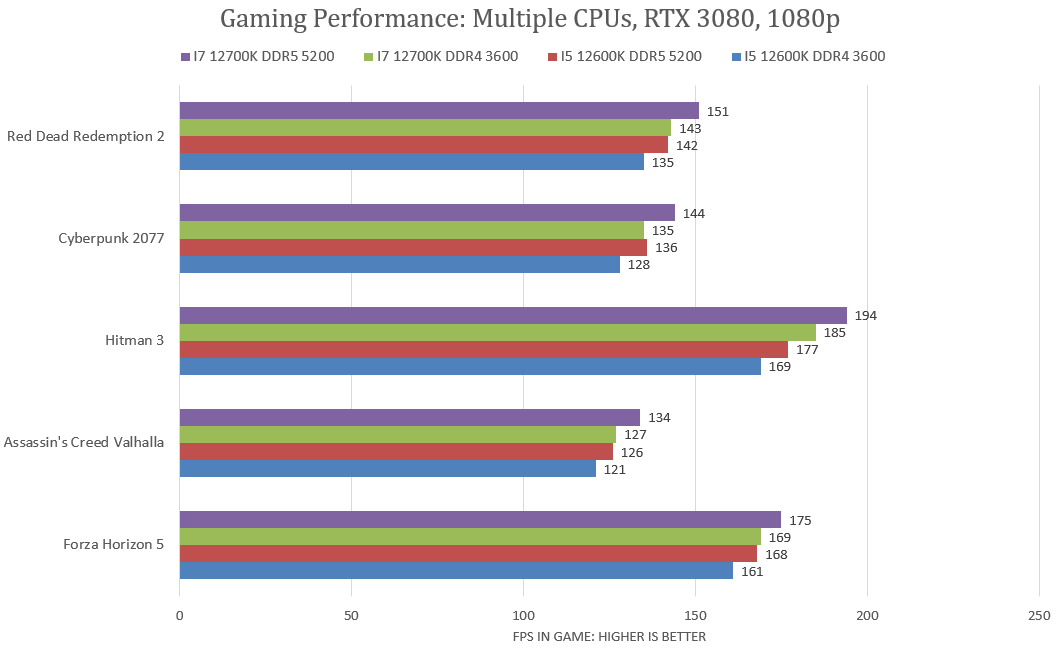
\includegraphics[width=13cm]{figures/Diagram Gaming Performance Multiple CPUs.png}
    \caption{Average performance with Intel Core i5 12600K and i7 12700K \parencite{youtube_test_i7+i5, youtube_test_i5}}
\end{figure}

As we can see in Figure 1, there are minor changes between the use of DDR4 and DDR5 inside a CPU configuration. We also see that at most of the games, the weaker i5 12600K with DDR5 RAM can on average compete with the stronger i7 12700K with DDR4 RAM. On average, the i5 12600K with DDR5 even beat the i7 12700k with DDR4 in Cyberpunk 2077 \parencite{youtube_test_i7+i5, youtube_test_i5}.
\\
We also wanted to know how much of a difference the RAM can make at only one CPU. That is why we searched for tests only regarding the Intel Core i9 12900K, the best CPU of Intel's 12th generation line-up. For these tests, two different RAM modules for each generation were used to see how much of a difference even inside a DDR generation it can make. The RAM that was used are DDR4 at 3200 MHz with a CAS latency of CL14 and 4000 MHz with a CAS latency of CL14, while the DDR5 modules are clocked at 4800 MHz and 6000 MHz and at CAS latencies of both CL36. The GPU that was used in these tests is an AMD Radeon RX 6900 XT, while the screen resolution stays the same as in the test of Figure 1.

\begin{figure}[H]
    \centering
    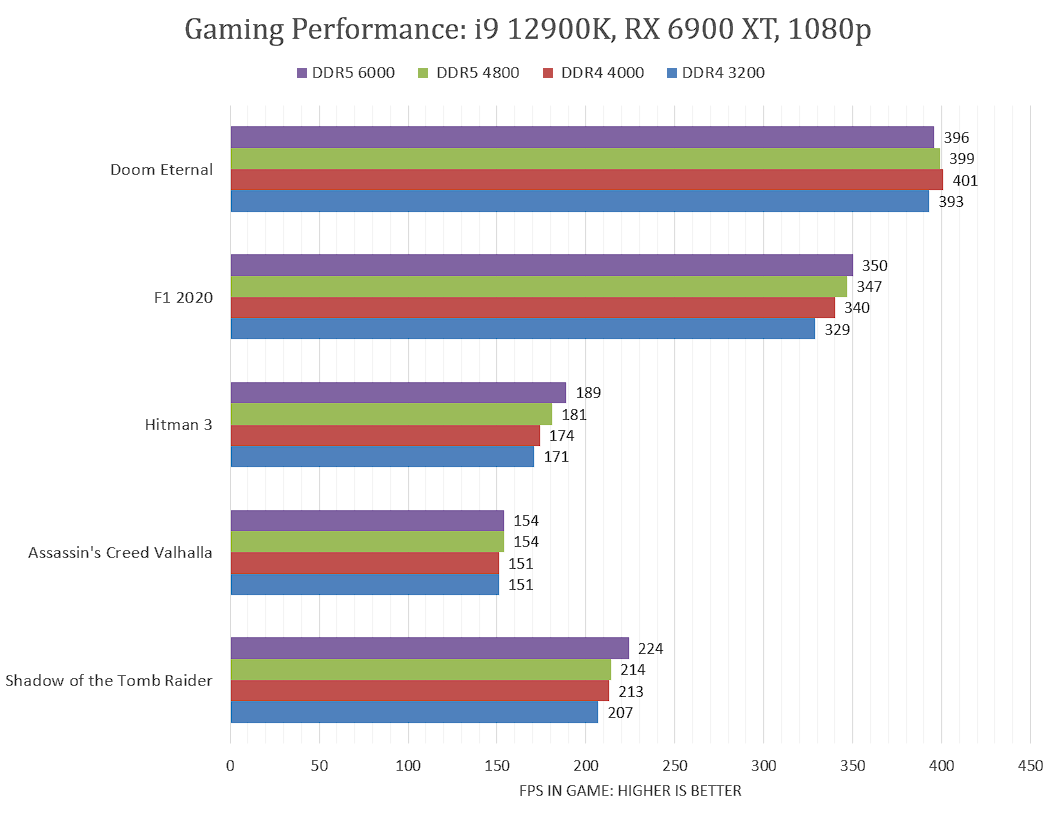
\includegraphics[width=13cm]{figures/Diagram Gaming Performance i9.png}
    \caption{Performance with Intel Core i9 12900K \parencite{12900k_gaming_and_work_benchmarks}}
\end{figure}

We can see in Figure 2, that with every RAM change, there is also an improvement in performance. What is a bit surprising, is that DOOM Eternal runs better at DDR4 RAM with a clock speed of 4000 MHz than DDR5 RAM as a whole \parencite{12900k_gaming_and_work_benchmarks}.
\\
\\
Because the gaming performance draws not the whole picture, we also took a look at synthetic benchmarks. In these benchmarks, only an Intel Core i9 12900K was used. Figure 3 shows the results of 3DMark. Here, 4 different RAM kits that were used, two kits for each generation.

\begin{figure}[H]
    \centering
    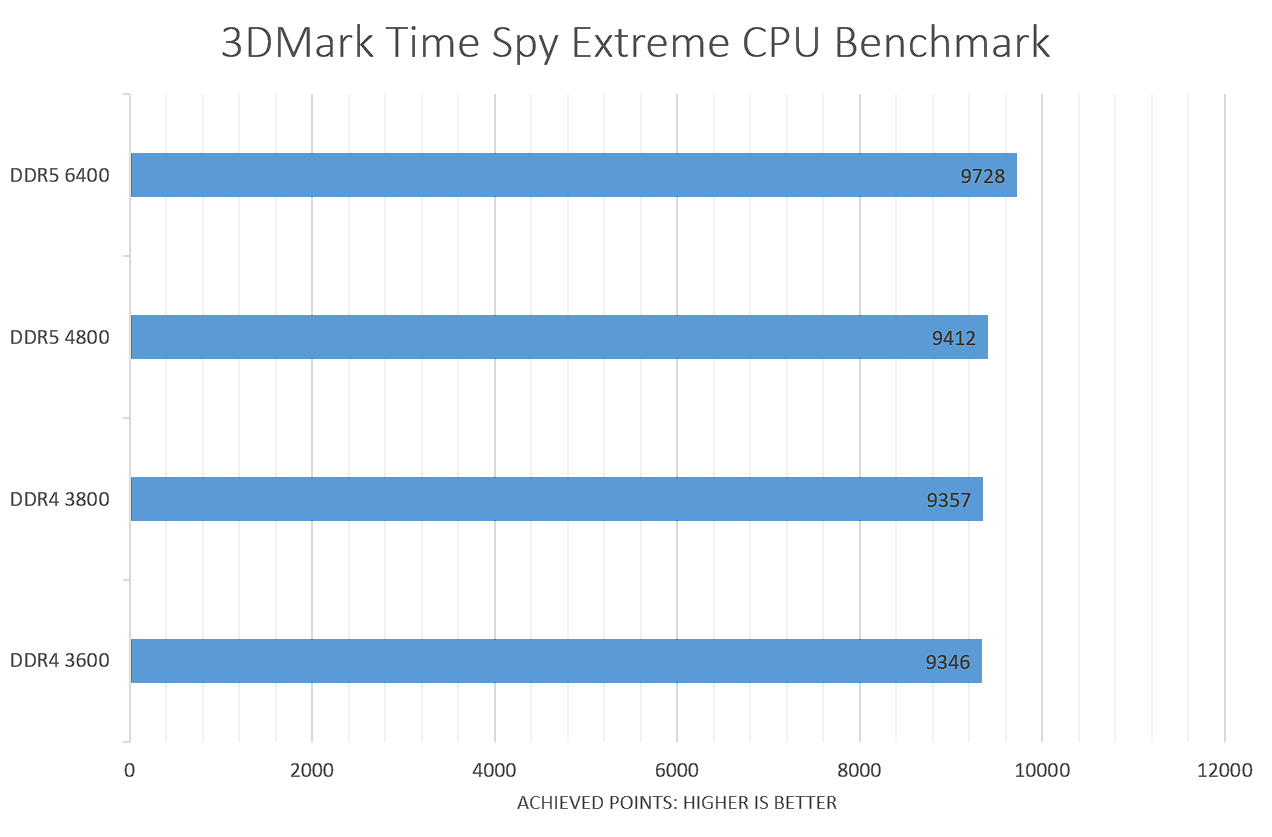
\includegraphics[width=13cm]{figures/Diagram 3DMark.png}
    \caption{Performance of i9 12900K in a general stress test \parencite{youtube_test_3dmark}}
\end{figure}

The RAM kits that were used are two DDR4 and two DDR5 kits. The DDR4 kits are having a frequency of 3600 MHz and 3800 MHz while both having a CAS latency of CL16, while the DDR5 kits are having a frequency of 4800 MHz and 6400 MHz and a CAS latency of CL40 for the 4800 MHz kit and CL38 for the 6400 MHz. As we have seen in the gaming comparison, each RAM step up again provides a small performance improvement, which is around 1\% - 4\% for each RAM step up. That means that the CPU can perform in a general stress test around 2\% - 3\% better when a fast DDR5 kit is used \parencite{youtube_test_3dmark}.
\\
\\
For a more specific test, the compressing and decompressing files with the 7-Zip application, the Intel Core i9 12900K was paired with a DDR4 kit with a frequency of 3600 MHz at a CAS latency of CL16 and a DDR5 kit with a frequency of 5200 MHz at a CAS latency of CL40. Figure 4 shows the compressing and decompressing rate in \gls{MB/s} of both tests.

\begin{figure}[H]
    \centering
    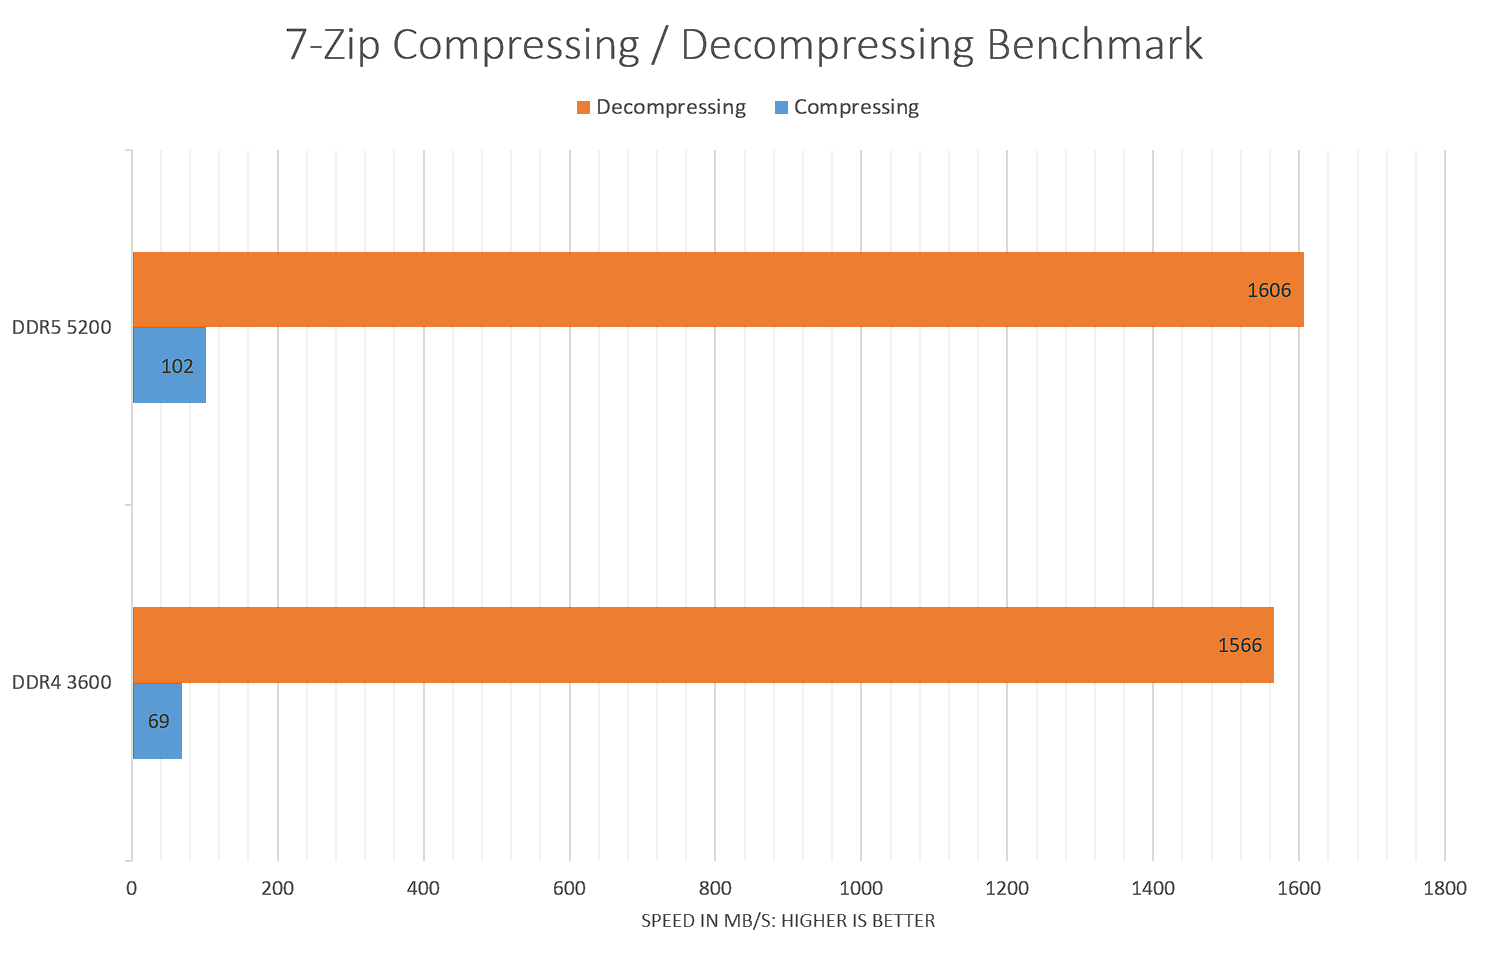
\includegraphics[width=13cm]{figures/Diagram 7-Zip.png}
    \caption{Compression and decompression test with 7-Zip \parencite{test_7zip}}
\end{figure}

As we can see in Figure 4, the tests show, that the CPU can perform around 45\% faster at compressing files when using the DDR5 kit, while performing around 3\% faster at decompressing files when using the DDR5 kit. This test respectively shows, when using DDR5 RAM, that the CPU is performing a bit faster in multithreaded workloads \parencite{test_7zip}.
\\
\\
Because these tests did not test for any creative work, we also included a test that benchmarks the performance of the system in Adobe Photoshop. This tool is called PugetBench, and it tests the encoding strength of the CPU, which is important for creative work like Adobe Photoshop or streaming on streaming services like Twitch \parencite{what_is_pugetbench}. For the tests, again an Intel Core i9 12900K with two RAM kits were used, one DDR4 kit at a frequency of 3200 MHz at a CAS latency of CL22, while the DDR5 kit runs at a frequency of 4400 MHz at a CAS latency of CL40. Figure 5 shows the results of said tests.

\begin{figure}[H]
    \centering
    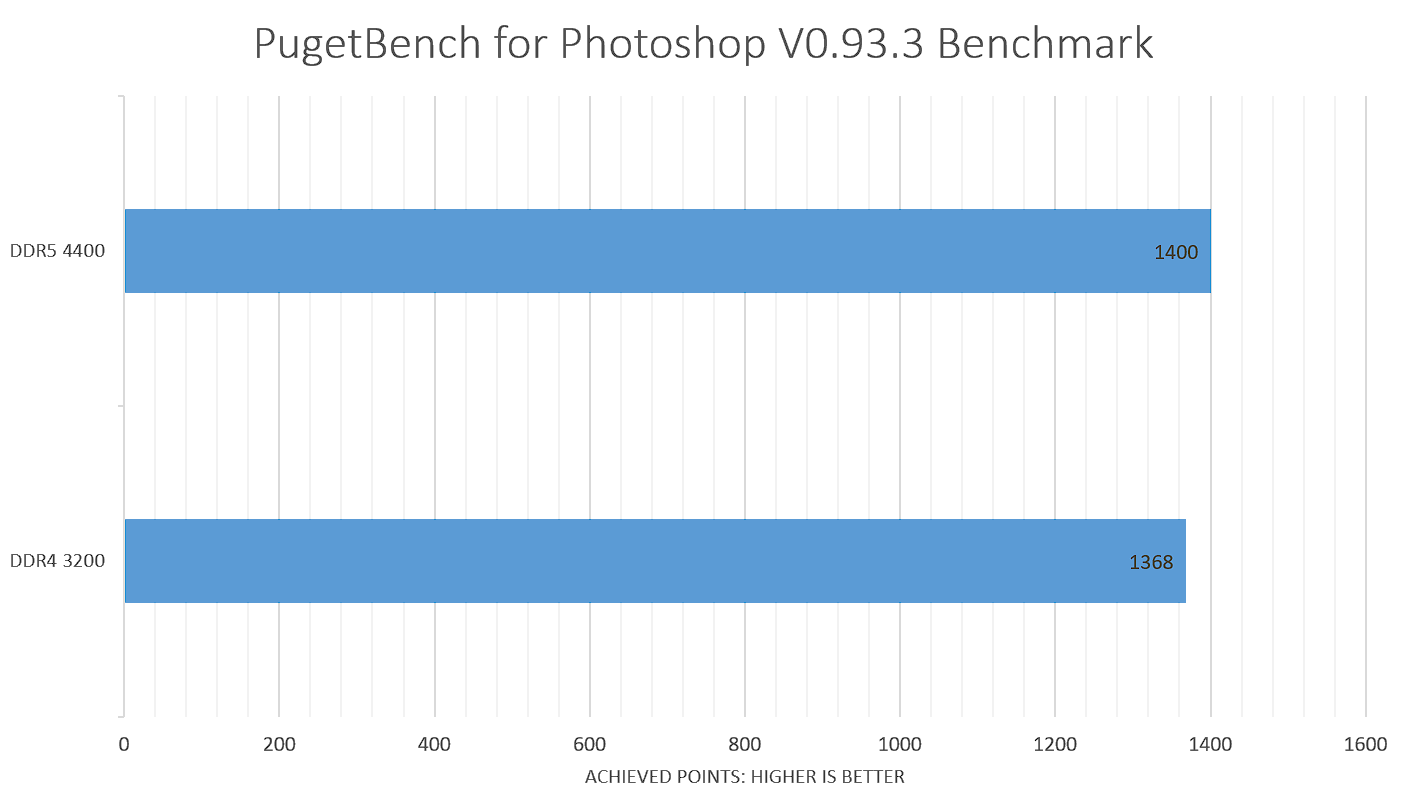
\includegraphics[width=13cm]{figures/Diagram PugetBench.png}
    \caption{Performance of i9 12900K in creative work \parencite{pugetbench_test}}
\end{figure}

Again, we can see a small 3\% increase in performance when using the DDR5 RAM kit. This means that if someone uses creative apps, like Adobe Photoshop or Blender, or is streaming on Twitch or another streaming platform, DDR5 can improve the performance a bit \parencite{pugetbench_test}.
\\
To conclude, when using DDR5, a mostly small improvement (1\% - 45\%) can be expected across the CPU.

\newpage

\subsection{Price-performance Comparison}

Now that we know the performance difference, we want to know if the price of DDR5 is changing over the year. Because DDR5 was firstly introduced at the end of 2021, there is not many data that can be used to define the price of that time. That is why Figure 6 shows the price of DDR5 only from March. The prices that are compared in Figure 6 are from RAM kits from the manufacturer Crucial. The first RAM kit is a 2 × 16 GB DDR4 RAM kit running at a frequency of 3200 MHz at a CAS latency of CL20, while the second RAM kit is a 2 × 16 GB DDR5 RAM kit running at a frequency of 4800 MHz at a CAS latency of CL40. Even though the retail price of the DDR4 kit is set at a price of €103.52 \parencite{Crucial_ddr4} and the DDR5 kit is set at a price of €148.74 \parencite{Crucial_ddr5}, vendors set their prices to how demanded the kits are.

\begin{figure}[H]
    \centering
    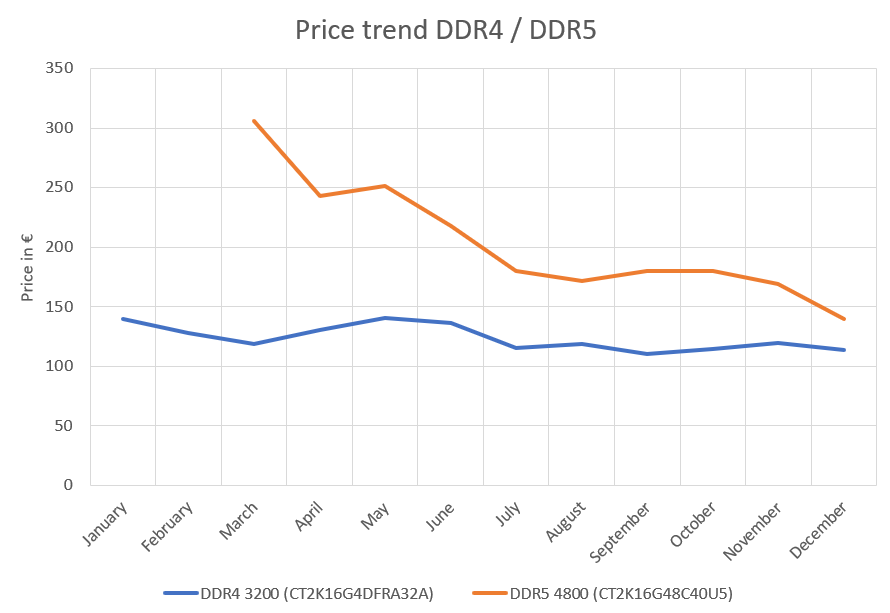
\includegraphics[width=13cm]{figures/Diagram Price Trend.png}
    \caption{Price trend of DDR4 kit and DDR5 kit in 2022 \parencite{Geizhals_ddr4, Geizhals_ddr5}}
\end{figure}

We see that DDR5 was at the beginning of 2022 very expensive. We also see, that the price for DDR5 has fallen, and at the end of 2022, the DDR5 kit costs half of what it would cost in March. These price changes did not affect the price trend of the DDR4 kit at all. It can be seen, that the price for the DDR4 kit did not change dramatically, like how the price of the DDR5 kit did. Still, the DDR5 kit costs around 16\% more than the DDR4 kit at the end of the year.
\\
\\
Performance and price are two separate categories, which have nothing to do with each other. However, with calculations, a connection between price and performance can be established. This helps to evaluate, if a specific configuration is worth the additional costs. In Table 2, we included first the average price of every kit that was used in the tests above. The rest data conclude how much performance someone per Euro in the tests above would get. As we can see in Table 2, the price-performance ratio is with DDR4 in almost every category higher than it is with DDR5, except in the 7-Zip Compress benchmark. Here, DDR5 provides a tiny bit more performance per Euro than DDR4. What this all means will be discussed in the next chapter. 

\begin{table}[H] 
    \centering
    \begin{tabular}{|m{5cm}|P{3cm}|P{3cm}|}
    \hline
                                             & \textbf{DDR4}  & \textbf{DDR5}    \\ \hline
    Average cost per used kit (Euro)         & 107,75         & 159,11           \\ \hline
    Games (FPS)                              & 3,715          & 1,306            \\ \hline
    3DMark (Points)                          & 86,789         & 60,147           \\ \hline
    7-Zip Decompress (MB/s)                  & 14,534         & 10,094           \\ \hline
    7-Zip Compress (MB/s)                    & 0,64           & 0,641            \\ \hline
    PugetBench (Points)                      & 12,696         & 8,799            \\ \hline
    
    \end{tabular}
    \caption{Performance per Euro ratio}
\end{table}